%hidelinks for hide color of clickable references
%scrreprt koma-script no idea what koma script does
\documentclass[hidelinks,12pt,a4paper, liststotoc, bibtotoc]{scrreprt}
%                     liststotoc,            % Tabellen & Abbildungsverzeichnis ins TOC 
%                     %idxtotoc,             % Index ins TOC 
%                     bibtotoc,               % Bibliographie ins TOC 
%                     bibtotocnumbered,    % Bibliographie im TOC nummeriert 
%                     %liststotocnumbered, % Alle Verzeichnisse im TOC nummeriert 

\usepackage[ngerman]{babel}
\usepackage[utf8]{inputenc}

%\usepackage[T1]{fontenc}
\usepackage{wrapfig}
\usepackage{amsmath}
\usepackage{amsfonts}
\usepackage{amssymb}
\usepackage{makeidx}
\usepackage{graphicx}
\usepackage{lmodern}
\usepackage{kpfonts}
\usepackage[doublespacing]{setspace}
\onehalfspacing
%\usepackage{fourier}
%\usepackage[left=2.5cm,right=2cm,top=4cm,bottom=4cm]{geometry}

% Beschreibund von Abbildungen NICHT einrücken 
\setcapindent{0pt}

%%Paket für Verweise auf bestimmte Seiten (klicken auf das Inhaltsverzeichnis)
\usepackage{hyperref}

%%Paket um die Zitierweise + Literaturverzeichnis einstellen zu können
\usepackage[style=authoryear-ibid,backend=biber]{biblatex}

%nicht anrücken nach absatz
\setlength{\parindent}{0pt}

%command um shell Kommandos schön darzustellen
\newcommand{\shellcmd}[1]{\indent\indent\texttt{\footnotesize\# #1}}

%%Paket für Kopf- und Fußzeile
\usepackage[]{scrlayer-scrpage}
%%Kopfzeile mit dem aktuellen Unterkapitel füllen
\automark{section}

\usepackage{lscape} % Querformat includegraphics

\pagestyle{scrheadings}

%%information for titlepage
\title{Titel der Arbeit}
\author{Autoren der Arbeit}
\date{\today}
%\thanks{Dankesworte}

%%bib-file einbinden
\addbibresource{Literatur.bib}

%%Zähler um am Ende auf der Bibliography Seite römisch weiter zählen zu können
\newcounter{pageNumberAfterContent}
\begin{document}

%Titelseite erstellen



%%Seitennummerierung neu beginnen, Zahlen [arabic], röm.Zahlen [roman,Roman], Buchstaben [alph,Alph]
\pagenumbering{Roman}


%Heißt erstelle ein Inhaltsverzeichnis
\tableofcontents



%\listoffigures

%\listoftables

\clearpage

%%Seitenzahl speichern
\setcounter{pageNumberAfterContent}{\value{page}}

\pagenumbering{arabic}

\clearpage
\chapter{Materialien und Grundlagen}

Zunächst werden für ein besseres Verständnis der Arbeit die eingesetzten Materialien und Grundlagen vorgestellt. Zu diesen zählen diverse Hardware, wie das verwendete Smartphone, das Ultraschallgerät oder der WLAN-Router, aber auch Software wie unter anderem die Entwicklungsumgebung oder das verwendete SDK (Software Development Kit). 

\section{Das LG G4}

Für eine zufriedenstellende Umsetzung der Anforderungen \textbf{(siehe Kapitel X)} muss das gewählte Smartphone über ein möglichst helles Display verfügen. Zudem sollte die Leistung des Prozessors ausreichend für eine Bildbearbeitung der einzelnen Videoframes sein, sodass es zu keinen Verzögerungen bei der Darstellung auf dem Smartphone kommt.
\\ 
\\
Wir haben uns aufgrund oben noch einmal kurz zusammengefasster Anforderungen für das Modell G4 der Marke LG entschieden.  Das Display des LG G4 ist ein AH-IPS (Advanced High Performance – In-Plane Switching) Display vom Typ Curved IPS Quantum Display. Die IPS Technologie verringert die Blickwinkelabhängigkeit des Kontrastes \footcite{LC-Schirme}. Das Display besitzt eine Diagonale von 14cm und eine Auflösung von 2560 x 1440 Pixel (Quad HD). Die Punktdichte beträgt entsprechend 538 ppi. Der Prozessor des Smartphones ist ein 6 Kern Qualcomm Snapdragon 808 mit einer Taktrate von 1,8 GHz. Es verfügt über einen Arbeitsspeicher von 3 GB. Das Betriebssystem des LG G4 ist ein natives Android der Version 5.1.\footcite{LGG4} 

\section{Android, Android SDK und Android Studio} \label{Android}

Android \footcite{Android} ist ein Betriebssystem für mobile Geräte wie Smartphones oder Tablets, ursprünglich entwickelt von der Firma Android, Inc., welche 2005 von Google aufgekauft wurde \footcite{AndroidHistory}. Mobile Anwendungen für Android Systeme werden in der Programmiersprache Java geschrieben und anschließend in Androids eigenes Format DEX (Dalvik Executable Format) konvertiert \footcite{AndroidCookbook}. Die Android UI Guidelines \footcite{AndroidGuidelines} geben Richtlinien für das Design der Benutzeroberfläche von Android Anwendungen vor.
\\
\\
Des Weiteren sind für Android Anwendungen unter anderem noch folgende Grundbedingungen formuliert, an welche sich bei der Planung der Anwendung gehalten wurde: Die Anwendung sollte einfach zu installieren, zu entfernen und zu updaten sein. Sie sollte ansprechend sein und die Anforderungen elegant umsetzen um auch bei vielen Features leicht bedienbar zu bleiben. Wichtig ist, dass die Anwendung stabil, skalierbar, bedienbar ist und angemessen auf Benutzereingaben reagiert.\footcite{AndroidCookbook}
\\
\\
Das Android SDK ist eine Entwicklungsumgebung für das Android Betriebssystem welches sich an Entwickler zur Erstellung von Android-Anwendungen wendet und ist für Windows, Linux und Mac OS verfügbar. Es benötigt für viele Hauptfunktionen ein JDK (Java Development Kit) \footcite{AndroidSDK}. Das SDK beinhaltet einen Emulator, der es möglich macht die Anwendung auch ohne angeschlossenes Smartphone zu testen. Als IDE (Integrated Development Environment) wurde Android Studio von uns genutzt, welches 2014 von Google veröffentlicht wurde und so Eclipse als primäre Entwicklungsumgebung für Android Anwendungen ablöste. Android Studio basiert auf der IntelliJ IDEA Community Edition von JetBrains. \footcite{AndroidOP} Es beinhaltet intuitive Tools, die die Erstellung einer grafischen Benutzeroberfläche nach den Android UI Guidelines \footcite{AndroidGuidelines} erleichtern. 

\section{GitHub}

Zum gemeinsamen Entwickeln an der mobilen Anwendung wurde ein kostenfreies Repository bei GitHub eingerichtet, welches integriert aus Visual Studio verwendbar ist. GitHub stellt für das gemeinsame Verwalteten von Repositories wichtige Funktionalitäten wie Forks (Abspaltungen) und Merges (Wiedervereinigungen) zur Verfügung. Auf diese Weise ist es dem Hauptverwalter, oder dem hauptverwaltenden Team möglich zu entscheiden, welche Änderungen von welchem Entwickler in das Projekt übernommen werden sollen. \footcite{GitHub}

\section{SonoScape S2}

Das für diese Arbeit eingesetzte Ultraschallgerät stammt von dem 2002 in Shenzhen, China gegründeten Unternehmen SonoScape Medical Corp. Zu den Produkten von SonoScape Medical Corp. zählen hauptsächlich Farb-Doppler Ultraschall Systeme, aber auch Endoskopie- und Elektrokardiographie-Systeme \footcite{SonoScape}.
\\
\\
In dieser Arbeit wurde das Modell S2 von SonoScape verwendet. Das Betriebssystem des Geräts ist ein modifiziertes Linux Ubuntu 10.04. Das Gerät verfügt über einen hochauflösenden 15" Weitwinkel LCD-Monitor. Es verfügt über eine Farbanzeige, was bei diesem Modell nicht standardmäßig ist. Die zwei Sondenanschlüsse mit Sondenhalter ermöglichen verschiedenste Anwendungen, wie unter anderem Abdominal, OB (Oberbauch), GYN (Gynäkologie), Gefäße, Urologie oder Small Parts. Die integrierte M-Tuning Technologie ermöglicht eine automatische B-Bild bzw. Doppler Optimierung. Die Bildfunktionen des SonoScape S2 sind B, B+B, B+M und 4B. Der integrierte Akku hat eine Stunde Laufzeit und die Anschlüsse des Geräts sind VGA, Video out, USB, S-Video, EKG Modul, DICOM 3.0. Zudem verfügt es über eine interne digitale Bildspeicherung. \footcite{SonoScapeS2}

\section{Der Teilerspiegel}

Ein Teilerspiegel reflektiert einen Teil des einfallenden Lichts transmittiert den anderen Teil. Auf diesem Wege ist es möglich, sowohl, was sich hinter dem Spiegel, als auch was sich vor ihm befindet zu sehen. Nur so kann der Effekt des optisch in den Körper projizierten Ultraschallbildes erzielt werden. Meist besteht ein solcher Spiegel auf der einen Seite aus einem dielektrischen Schichtensystem oder einer dünnen Metallbeschichtung und auf der anderen aus einer reflexionsvermindernden Beschichtung. Der für diese Arbeit gewählte Spiegel ist ein Zwei-Wege-Acryl-Spiegel mit den Maßen 120 x 184mm. Er hat eine Dicke von 6mm. \footcite{Teilerspiegel}

\section{Die Halterung}

Damit mit dem Smartphone und dem Teilerspiegel das Ultraschallbild in den Patientenkörper hinein projiziert werden kann ohne den Arzt bei seiner Arbeit zu behindern, ist es notwendig sowohl Smartphone als auch Spiegel im richtigen Winkel zueinander an den Ultraschallkopf zu befestigen \textbf{(siehe Kapitel X)}.
\\
\\
Um eine solche Halterung zu bauen, wurden Modelliermasse, Kabelbinder, eine Hülle passend für das LG G4, Metallwinkel und Heißkleber verwendet. Die Modelliermasse, die hierfür verwendet wurde, ist die FIMO Modelliermasse der Firma STAEDTLER. Sie ist weich und formbar und lässt sich nach der Modellage Ofen aushärten \footcite{FIMO}.

\section{Das Phantom} \label{Phantom}

Für die Evaluierung der Arbeit \textbf{(siehe Kapitel X)} wurde ein Phantom angefertigt. Dieses Phantom besteht aus einer Gelatineplatte, in der sich zwei 1-Cent Münzen befinden. Eben genannte Gelatineplatte besteht aus 100ml Wasser, 50ml Isopropyl-Alkohol, 50ml Glycerin und brauner Lebensmittelfarbe.

\section{YUV-Farbmodell} \label{YUV}

Bei dem YUV-Farbmodell wird die Bildhelligkeit von der Farbdifferenz getrennt. Hierbei beschreibt die Y-Komponente die Luminanz und die U- und V-Komponenten die Chrominanz. Historisch sind die YUV-Modelle eng mit der Entwicklung des Farbfernsehens verknüpft, da man ein Verfahren benötigte, durch zusätzliche Übertragung der Farbkomponente das Farbfernsehen bei Weiterbenutzung der alten Schwarzweiß-Empfänger zu ermöglichen. \footcite{YUV_Farbmodell}
\\
\\
Die Aufteilung der einzelnen Komponenten in einem einzelnen Frame im NV12-Format, welches Bilder im YUV-Farbmodell darstellt, lässt sich wie in Abbildung \ref{fig:YUV_Frame} vorstellen:


\begin{figure}[h]
	\centering
	\includegraphics[width=0.5\textwidth]{Bilder/Materialien_und_Grundlagen/YUV_Frame.PNG}
	\caption{Frame im NV21-Format (YUV-Farbmodell)}
	\label{fig:YUV_Frame}
\end{figure}

~\\
Wie man unschwer erkennen kann, befinden sich die Informationen bezüglich der Luminanz in den ersten zwei Dritteln des Frames. Um aus einem Frame im YUV-Format ein Schwarzweißbild zu erzeugen, bräuchte man entsprechend nur diese Komponenten. 
\\
\\
Überführt man ein oben gezeigtes Frame (\ref{fig:YUV_Frame}) in ein eindimensionales Array, erhält man entsprechend folgende Aufteilung: 

\begin{figure}[h]
	\centering
	\includegraphics[width=1\textwidth]{Bilder/Materialien_und_Grundlagen/YUV_Array.PNG}
	\caption{Eindimensionales Array entsprechend eines Frames im NV21-Format (YUV-Farbmodell)}
	\label{fig:YUV_Array}
\end{figure}

\section{RGB-Farbmodell und Konvertierung} \label{YUV_RGBKonvert}

Das RGB-Farbmodell ist ein additives Farbmodell, bei dem die Farben durch Mischung der Grundfarben Rot, Grün und Blau dargestellt werden. Ein digitales Farbbild besitzt dabei für jeden Bildpunkt drei Werte, die die Anteile an Rot, Grün und Blau beschreiben. Der Wertebereich erstreckt sich dabei üblicherweise zwischen 0 und 255. Man kann sich dies als drei M x N Matrizen vorstellen: pro Grundfarbe eine Matrix, in der für jeden Pixel der Anteil der entsprechenden Grundfarbe gespeichert ist (siehe Abbildung \ref{fig:RGB-Matrizen}). \footcite{MTI2}


\begin{figure}[h]
	\centering
	\includegraphics[width=0.55\textwidth]{Bilder/Materialien_und_Grundlagen/RGB_Matritzen2.png}
	\caption{Farbmatrizen des RGB-Farbmodells}
	\label{fig:RGB-Matrizen}
\end{figure}

Um die RGB-Werte eines Pixels aus einem Frame im YUV-Format zu ermitteln, müssen die entsprechenden Luminanz- und Chrominanzwerte dieses Pixels aus dem YUV-Frame ermittelt und in RGB-Werte umgerechnet werden. Bei der Wahl der Formel zur Umrechnung vom YUV-Farbformat in ein RGB-Farbformat ist zu beachten in welchem exakten Format sich das Ausgangsframe befindet. Die Frames, die in dieser Arbeit konvertiert werden mussten, befanden sich im Format YUV420, weshalb sich folgende Konstanten für die Umrechnungsformeln für die einzelnen Werte R, G und B eines Pixels ergaben \footcite{Konvertierung}:
\\

$R = clamp(Y + 1.402 \times V) $\\
$G = clamp(Y - 0.344 \times U - 0.714 \times V) $\\
$B = clamp(Y + 1.772 \times U) $\\
\chapter{Bildakquise und Datenaufbereitung}
Eine der grundlegenden Funktionalitäten des Projektes ist die Anzeige der Bilddaten des Ultraschallgerätes auf einem Smartphone Display. Dieser Prozess kann auf verschiedene Arten implementiert werden, welche unterschiedliche Vor- und Nachteile haben. Alle Ansätze haben jedoch eine grundlegende Abfolge von Arbeitsschritten gemein (siehe Abbildung \ref{fig:Bildakquise_schritte}).\\

\begin{figure}[h]
	\centering
	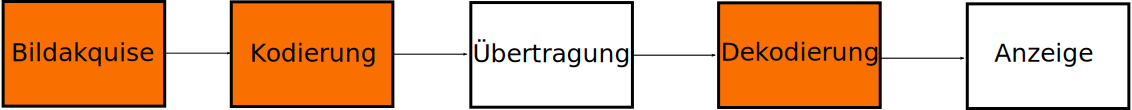
\includegraphics[width=1\textwidth]{Bilder/BildakquiseUndDatenaufbereitung/Bildakquise_schritte.pdf}
	\caption{Prozessschitte zur Anzeige der der Bilddaten auf dem Zielgerät. Die in diesem Kapitel behandelten Schritte sind farbig markiert.}
	\label{fig:Bildakquise_schritte}
\end{figure}

Im vorliegenden Kapitel wird primär auf die Schritte \textit{Bildakquise}, \textit{Kodierung} sowie \textit{Dekodierung} eingegangen, da die Implementierungen dieser Funktionalitäten direkt voneinander abhängen und somit nicht getrennt betrachtet werden können. Die Datenübertragung und Anzeige der Bilddaten bleiben hingegen unbeeinflusst von den genannten Prozessschritten und werden somit gesondert behandelt.\\

\section{Bildakquise}
Der Prozesschritt der Bildakquise beinhaltet die Ermittlung der Bilddaten von dem Quellgerät. Dabei können, je nach vorhandener Hard- und Softwarekonfiguration verschiedene Ansätze verfolgt werden.\\
\\
Ein möglicher Ansatz ist die Verwendung eines Hardwareadapters (\glqq FrameGrabber\grqq), welcher die Videosignale des Quellgerätes über dessen Videoausgang entgegennimmt und über eine Datenschnittstelle einem verarbeitenden Gerät zur Verfügung stellt. Ein Vorteil dieser Vorgehensweise ist die Simplizität in Bezug auf das Quellgerät. Da das Videosignal über bereits vorhandene, standardisierte Schnittstellen übertragen wird, muss keine Veränderung an der Software des Gerätes vorgenommen werden.\\
Im Gegenzug dazu wird jedoch ein weiteres Gerät, welches die Bilddaten entgegennimmt und verarbeitet, benötigt. Damit steigt die Gesamtkomplexität des Systems erheblich an, da statt einem Quell- und einem Zielgerät nunmehr ein Quellgerät, ein Zwischengerät zur Verarbeitung und ein Zielgerät benötigt werden.\\

\begin{figure}[h]
	\centering
	\includegraphics[width=1\textwidth]{Bilder/BildakquiseUndDatenaufbereitung/Bildakquise_ansatz1.pdf}
	\caption{Bildakquise mittels eines FrameGrabbers}
	\label{fig:Bildakquise_ansatz1}
\end{figure}

~\\
Statt der Nutzung eines FrameGrabbers zur Aufnahme der Bilddaten kann auch eine Software, welche die Daten direkt auf dem Ultraschallgerät  aufnimmt und aufbereitet, genutzt werden. Hierzu muss jedoch direkter Zugriff auf das Betriebssystem des Ultraschallgerätes erlangt werden, was sich bei proprietären, geschlossenen Systemen schwierig gestalten kann. Des Weiteren muss die Systemleistung des Quellgerätes ausreichen, um neben der eigentlichen Bildverarbeitung, welche für die Aufnahme des Ultraschallbildes durchgeführt wird, auch noch die Bildakquise und Datenaufbereitung durchzuführen.\\
Der Vorteil dieses Ansatzes im Vergleich zur Nutzung eines FrameGrabbers ist der Wegfall von zwei Hardwarekomponenten im Gesamtsystem: Der FrameGrabber und die Hardware zur Zwischenverarbeitung entfallen, da die entsprechenden Arbeitsschritte direkt auf dem Ultraschallgerät durchgeführt werden können.

\section{Kodierung}
Bei der Kodierung werden die zuvor aufgenommen Bilddaten aufbereitet, um die Übertragung über einen beliebigen Datenkanal zu erleichtern. Dies ist vor allem notwendig, da die Datenmenge der unbehandelten Bilddaten zu hoch für eine Übertragung mittels eines kabellosen Mediums ist.  Wird die Framerate\footnote{Framerate bezeichnet die Anzahl der angezeigten Bilder pro Sekunde} auf 30 FPS\footnote{Frames per second - Bilder pro Sekunde}, die Bildauflösung auf $1024*768$ Pixel und die Farbtiefe auf drei Bytes pro Pixel festgelegt, ergibt sich eine erforderliche Datenrate von
\begin{equation}
D_r=1024*768*3*30=67.5 MByte/s.
\end{equation}
Wenn als Übertragungsmedium WLAN genutzt wird und der 802.11ac\footcite{WIFIStandard} Standard vorausgesetzt werden kann, ist bei einer üblichen Kanalbreite von 20 MHz eine maximale Übertragunsgrate von $96.3 Mbit/s$ oder $12 MByte/s$ möglich. Folglich können die Daten nicht ohne vorherige Kompression übertragen werden.

\section{Dekodierung}
Die Dekodierung rekonstruiert aus dem übertragenen Datenstrom die ursprünglichen Frames und gibt sie an zur Weiterverarbeitung und Anzeige frei. Dieser Prozessschritt wird auf dem Smartphone durchgeführt, da er erst nach der Datenübertragung stattfinden kann.

\section{Implementierung mit FFmpeg}
Im Verlaufe des Projektes wurden zwei verschiedene Ansätze implementiert und getestet. Bei dem ersten Ansatz wurden die Schritte der Bildakquise und Kodierung unter Zuhilfenahme der FFmpeg-Bibliothek\footcite{FFmpeg} realisiert, während zur Dekodierung unter anderem die Android MediaCodec Api\footcite{AndroidMediaCodec} genutzt wurde.\\
Die FFmpeg-Bibliothek bietet die Möglichkeit, über einen Kommandozeilenbefehl den aktuellen Bildschirminhalt als Videostream abzugreifen sowie die entstehenden Daten mit diversen Videocodecs zu kodieren. Der resultierende Datenstrom kann über die unter Linux vorhandene Pipe-Funktionalität in einen gesonderten Prozess umgeleitet werden, welcher die Übertragung bewerkstelligt.\\
\begin{figure}[H]
	
\includegraphics[width=1\textwidth]{Bilder/BildakquiseUndDatenaufbereitung/ffmpeg_befehl1.pdf}
	\caption{FFmpeg-Befehl zur Aufnahme und Speicherung des Bildschirminhaltes.}
	\label{fig:FFmpeg_befehl1}
\end{figure}

Ein beispielhafter FFmpeg-Befehl, welcher den Bildschirminhalt aufnimmt und in einer Datei abspeichert, kann Abbildung \ref{fig:FFmpeg_befehl1} entnommen werden. Es werden fünf Parameter angegeben, welche zur Ausführung des Befehls notwendig sind:
\begin{enumerate} 
	\item Der Schalter \textit{-s} legt die Auflösung des Quellmaterials fest. 
	\item Der Schalter \textit{-framerate} legt die Framerate fest.
	\item Der Schalter \textit{-f} legt die Videoquelle fest. Im gegebenen Fall ist die Quelle  das \textit{x11grab}-Device, welches unter Linux den Bildschirminhalt aufnimmt.
	\item Der Schalter \textit{-i} legt den Abschnitt, welcher abgefilmt werden soll, fest. Da der gesamte Bildschirm des Ultraschallgerätes aufgenommen werden soll, wird die linke obere Ecke des Bildschirms als Startpunkt angegeben.
	\item Die letzte Option gibt den Namen der Ausgabedatei an. 
\end{enumerate}

\subsection{Auswahl eines Videocodecs}
Die FFmpeg-Bibliothek unterstützt eine große Anzahl unterschiedlicher Videocodecs zur Kompression des Quellmaterials. Da die Dekodierung des Datenstroms auf dem Smartphone möglichst schnell und ressourcenschonend ablaufen soll, bietet es sich an, die vorhandene Hardwareunterstützung des Gerätes zu Nutzen. Hierbei wird die Dekodierung von einem dedizierten Hardwareschaltkreis durchgeführt, was die CPU des Smartphones entlastet und den Prozess deutlich beschleunigt. Die Anforderung der Hardwarebeschleunigung schränkt die Auswahl der möglichen Videocodecs deutlich ein.\\
Nach diversen Tests mit dem zur Verfügung stehenden Smartphone fiel die Wahl auf den H.264\footcite{H264} Videocodec, da dieser sowohl eine ausreichende Kompressionsrate bietet, als auch von der FFmpeg-Bibliothek sowie dem Smartphone-Decoder unterstützt wird.\\
Als Pixelformat wurde das NV12-Format\footcite{NV12} gewählt, da dieses die beste Unterstützung seitens des Smartphones aufwies.\\

\begin{lstlisting}[caption=Endgültiger FFmpeg-Konsolenbefehl zur Videoaufnahme, label=lst:ffmpeg_befehl, language=Java]
ffmpeg -s 1024x768 -framerate 15 -f x11grab -i :0.0 -pix_fmt nv12 
-c:v libx264 -x264opts keyint=10:min-keyint=10:scenecut=-1 
-b:v 6000000 -f h264 pipe:| videostream.bin
\end{lstlisting}

~\\
Dem Listing \ref{lst:ffmpeg_befehl} ist der endgültige Befehl zur Aufnahme des Live-Videos zu entnehmen. Zusätzlich zu dem zuvor dargestellten Befehl in Abbildung \ref{fig:FFmpeg_befehl1} wurden noch Schalter für das Pixelformat, den Videocodec sowie dessen Konfiguration angegeben. Über den \textit{pipe}-Ausdruck wird der gesamte Datenstrom umgeleitet und kann somit von einer beliebigen Software über den Standardinput ausgelesen und übertragen werden.

\subsection{Nutzung des MediaCodec}
Zur Dekodierung der Daten kann die Android MediaCodec Api genutzt werden. Diese stellt sicher dass die Verarbeitung der komprimierten Videodaten hardwarebeschleunigt über den dedizierten Schaltkreis des Gerätes stattfindet. \\

\begin{figure}[h]
	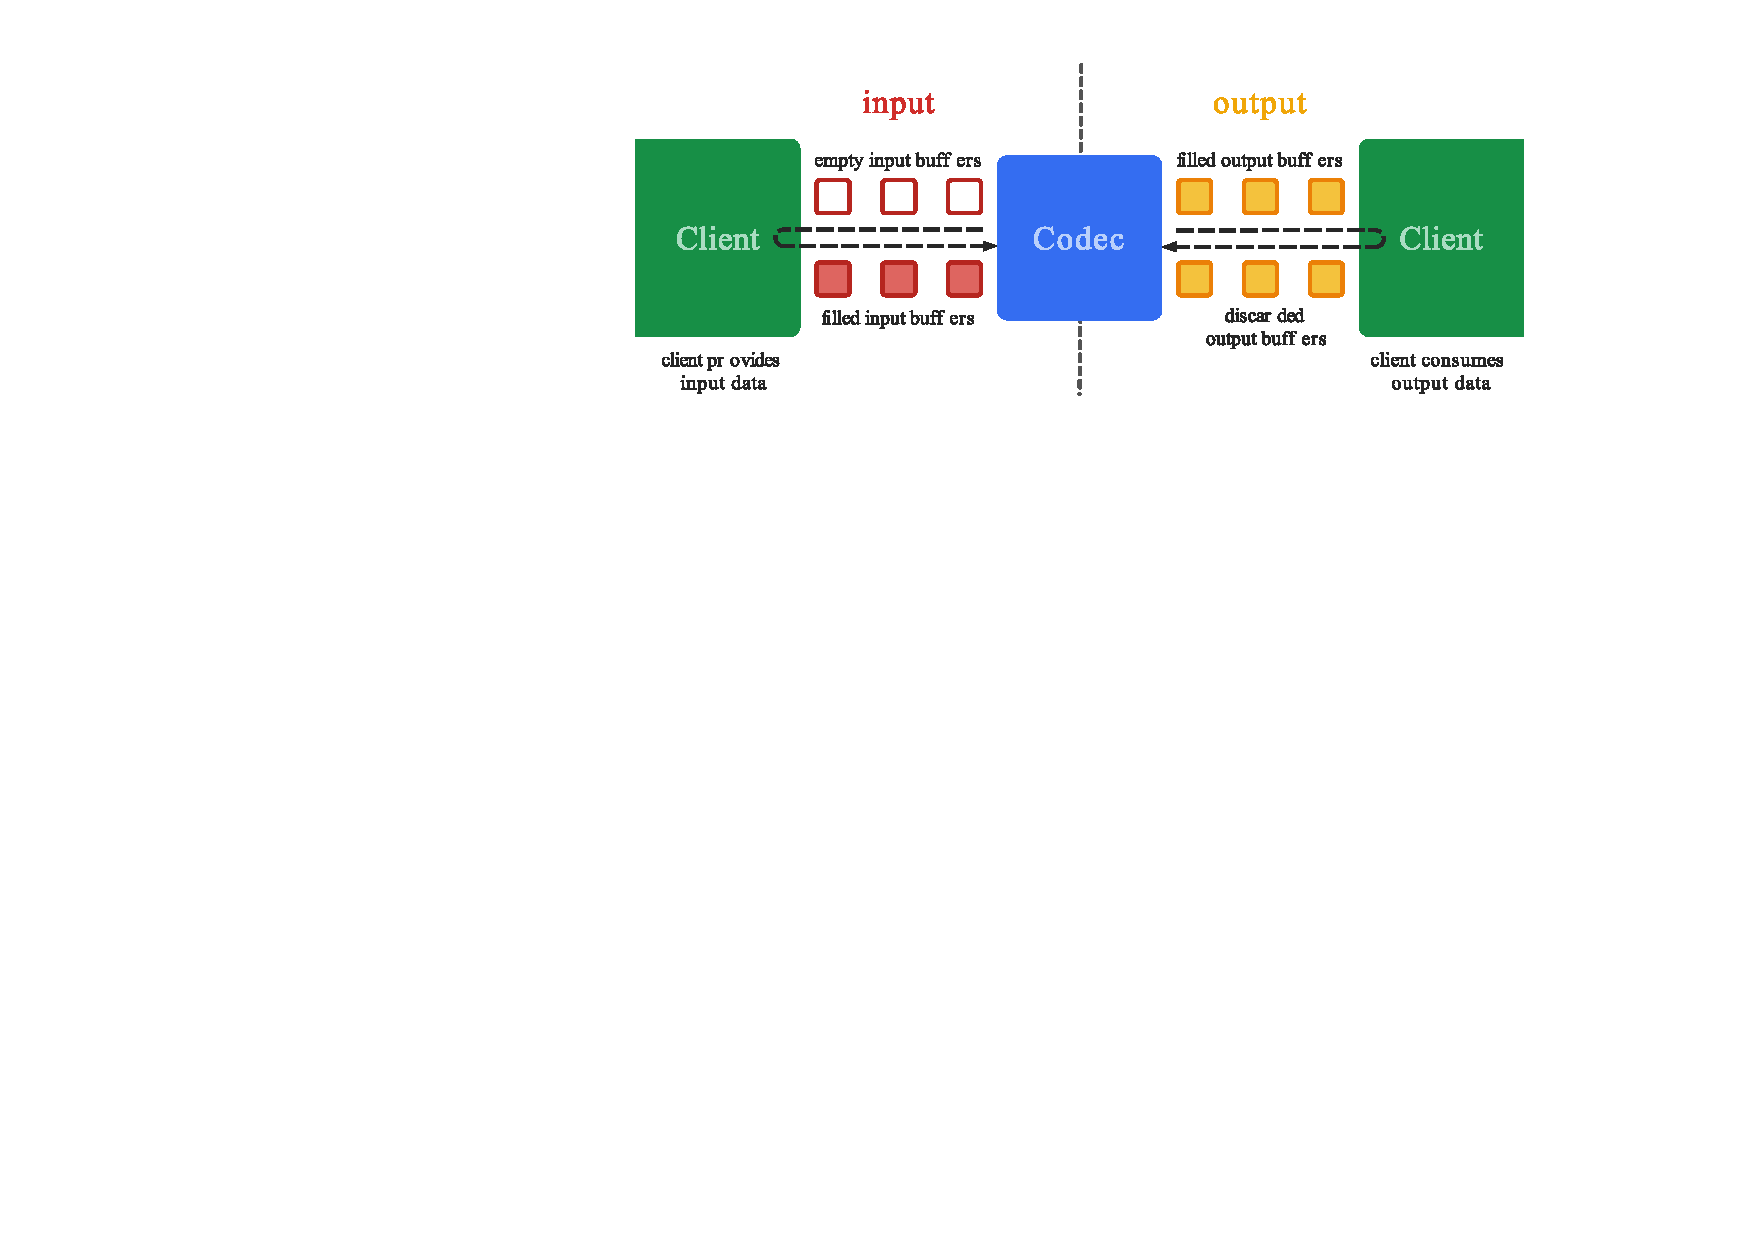
\includegraphics{Bilder/BildakquiseUndDatenaufbereitung/mediacodec.pdf}
	\caption[Nutzung der Android MediaCdec Api]{Nutzung der Android MediaCodec Api\footnotemark}
	\label{fig:media_codec}
\end{figure}
\footnotetext{\cite{AndroidMediaCodec}}
Die MediaCodec Api wird genutzt, indem die komprimierten Rohdaten Paketweise über Eingabepuffer an den Codec übertragen werden. Nach der Dekodierung werden die resultierenden Frames über die vom Codec zur Verfügung gestellten Ausgabepuffer ausgelesen und angezeigt.\\
Da die Daten als kontinuierlicher Datenstrom an das Smartphone gesendet werden, müssen sie vor der Übergabe an den MediaCodec in einzelne Pakete eingeteilt werden. Dabei ist es wichtig, dass die Pakete die erwartete Struktur und den erwarteten Inhalt aufweisen. Diese Eigenschaften sind von dem verwendeten Codec abhängig.\\
 In der vorliegenden Implementierung wurde als Übertragungsformat für die Rohdaten das Annex-B Format genutzt, bei welchem die Daten in sogenannte NALUs\footnote{Network Access Layer Unit} eingeteilt werden. Für den H.264 Codec entspricht somit ein Paket einer NALU.\\
\begin{figure}[H]
	\includegraphics{Bilder/BildakquiseUndDatenaufbereitung/NALUs.png}
	\caption{Rohdaten mit Delimitern.}
	\label{fig:nalus_delimiter}
\end{figure}
In dem Datenstrom sind die einzelnen NALUs durch eine festgelegte Bitfolge ("`Delimiter") voneinander getrennt. Im Hexadezimalsystem kann der Delimiter als \textit{00 00 00 01} oder alternativ mit einer Länge von drei Bytes als \textit{00 00 01} dargestellt werden. Beide Varianten sind dem Annex-B Standard zufolge gültige Delimiter.\\

\subsection{Verarbeitung des Datenstroms}
Zur korrekten Nutzung des MediaCodec muss der Rohdatenstrom also anhand der Delimiter in Echtzeit in einzelne NALUs aufgeteilt werden, welche darauffolgend in die Eingabepuffer des Codec gefüllt werden können. In der Implementierung sind dafür zwei Interfaces vorgesehen.\\
\clearpage
\textbf{INalUExtractor}\\
Das INalUExtractor-Interface stellt die Funktion \textit{extractNalUs()} zur Verfügung, welcher ein Byte-Array und die länge der enthaltenen Daten in Bytes übergeben werden kann. Das Ergebnis der Methode ist eine Liste von Byte-Arrays, die jeweils einegültige NALU enthalten und direkt dem MediaCodec-Eingabepuffer übergeben werden können. Sollten in den Übergebenen Daten unvollständige NALUs vorhanden sein (bspw. wenn der gelesene Block des Datenstroms nicht mit einem vollständigen Delimiter endet), werden diese Daten vorgehalten und beim nächsten Aufruf der Methode verarbeitet.\\
Somit ermöglicht eine gültige Implementierung des Interfaces die kontinuierliche Übergabe von beliebig langen Datenblöcken, welche dann in gültige NALUs aufgeteilt werden.\\
\begin{lstlisting}[caption=Definition des INaluUExtractor-Interface, label=lst:i_nalu_extractor, language=Java]
public interface INalUExtractor
{
    List<byte[]> extractNalUs(byte[] data, int length);
}
\end{lstlisting}
~\\
\\
\textbf{INalUSplitter}\\
Das INalUSplitter-Interface wird von der Implementierung des INalUExtractor-Interfaces genutzt, um einen Datenblock zu einem \textit{NalUSplitResult} zu verarbeiten. Es definiert die Methode \textit{splitBlock()} welche ein Byte-Array sowie die Länge der enthaltenen Daten erwartet und das Ergebis der Operation als \textit{NalUSplitResult} zurück gibt.

\begin{lstlisting}[caption=Definition der NalUSplitResult-Klasse, label=lst:nalu_split_result, language=Java]
public class NalUSplitResult
{
    private byte[] partialStartPart;
    private List<byte[]> completeNalUs;
    private byte[] partialEndPart;
    
    // Getter und Setter...
}
\end{lstlisting}

Ein \textit{NalUSplitResult} repräsentiert einen Datenblock, aufgeteilt in drei Komponenten. Das Feld \textit{partialStartPart} enthält die Bytes einer unvollständigen NALU zu beginn des Datenblockes. Eine solche NALU entsteht, wenn der vorherige Datenblock nicht mit einer vollständigen NALU endet und somit der aktuelle Datenblock nicht mit einem gültigen Delimiter beginnt.\\
Das Feld \textit{completeNalUs} enthält alle vollständigen, gültigen NALUs, die in dem übergebenen Datenblock vorhanden sind. Das Feld \textit{partialEndPart} enthält die Bytes, welche am Ende eines Datenblockes liegen aber nicht eindeutig eine vollständige NALU repräsentieren.\\
Die NalUSplitResult-Instanzen, welche für die Datenblöcke generiert werden, werden vom \textit{NalUExtractor} genutzt, um die unvollständigen Datenblöcke zusammenzuführen und einen kontinuierlichen Strom gültiger NALUs zu erzeugen.\\
\begin{lstlisting}[caption=Definition des INaluUSplitter-Interface, label=lst:i_nalu_splitter, language=Java]
public interface INalUSplitter 
{
    NalUSplitResult splitBlock(byte[] block, int length);
}
\end{lstlisting}

\subsection{Konfiguration des MediaCodec}
Zusätzlich zu den Datenpaketen, welche von der MediaCodec-Api erwartet werden, müssen noch weitere Konfigurationen zur erfolgreichen Nutzung des Codecs vorgenommen werden. Dazu gehören die Angabe des MIME-type des vorhandenen Videoformates und das Setzen der SPS\footnote{Sequence Parameter Set, enthält Informationen über den Aufbau des Videostreams} und PPS\footnote{Picture Parameter Set, enthält Informationen über die Konfiguration der einzelnen Frames.} Felder des Codecs.\\
 Diese Konfigurationen werden vor dem Start des Decoding-Prozesses vorgenommen. Die Datenübergabe an den Eingabepuffer und das Auslesen der Daten aus dem Ausgabepuffer erfolgt schließlich über Callback-Funktionen, welche für den Codec registriert werden müssen. \\
\\
Die Bytefolgen für die SPS- und PPS-Felder können ermittelt werden, indem gewisse NALUs eines Streams mit der gewünschten Konfiguration im Annex-B Format manuell analysiert werden. Jede NALU hat einen Typen, welcher über das erste Byte nach dem Delimiter festgelegt wird. Kommt in dem Stream eine NALU mit der Bitfolge \textit{0x67} (in Hexadezimaldarstellung) vor, handelt es sich um das SPS-Feld. Die Bitfolge \textit{0x68} signalisiert das PPS-Feld. 

\begin{lstlisting}[caption=Konfiguration des MediaCodec, label=lst:config_media_codec, language=Java]

private static final String MIME_TYPE = "video/avc";
private static final int WIDTH = 1280;
private static final int HEIGHT = 720;

private void configureCodec()
{
	codec = MediaCodec.createDecoderByType(MIME_TYPE);
	MediaFormat format = MediaFormat.createVideoFormat(MIME_TYPE, WIDTH, HEIGHT);
	byte[] sps = {  //...SPS-Bytes...};
	byte[] pps = { //...PPS-Bytes...};
	format.setByteBuffer("csd-0", ByteBuffer.wrap(sps));
	format.setByteBuffer("csd-1", ByteBuffer.wrap(pps));
	codec.configure(format, null, null, 0);
	//... Registrierung der Callbacks...
	codec.start();
}
\end{lstlisting}

\subsection{Performance und Funktionalität}
Die Implementierung mit den vorgestellten Methoden und Ansätzen funktionierte auf den Testgeräten nur eingeschränkt. Die Performance war zwar, sowohl auf dem Ultraschallgerät als auch auf dem Smartphone, sehr zufriedenstellend und das Datenaufkommen minimal, die Latenz der Gesamtlösung lag jedoch bei mehr als 2000 mS. Eine Echtzeitanwendung ist damit nur sehr eingeschränkt möglich, da Veränderungen des Ultraschallbildes erst mit einer großen Verzögerungen auf dem Smartphone angezeigt werden.\\
Die Latenz konnte auch durch Die Nutzung anderer alternativer Übertragungsformen und Videocodecs nur unzureichend verringert werden, da alleine das \textit{x11grab}-Device zur Aufnahme des Bildschirminhaltes eine Latenz von 800 mS erzeugte. \\

\section{Implementierung mit X11Lib und LZ4}
Da die Implementierung mit Hilfe der FFmpeg-Bibliothek eine zu hohe Latenz aufwies, musste eine Alternative gefunden werden. Bei der Konzeption stand, neben den schon zuvor ermittelten Anforderungen an die Performance und das Datenaufkommen, vor allem die Latenz im Mittelpunkt.\\ Es musste also für jeden Prozessschritt eine Implementierung geschaffen werden, welche innerhalb weniger Millisekunden ausgeführt werden kann um in der Summe auf eine Gesamtdauer von weniger als 200 mS zu kommen. 

\subsection{Bildakquise mit X11Lib}
X11Lib ist eine C++-Bibliothek, welche den direkten Zugriff auf Bilddaten des Linux-Grafiksystems ermöglicht. Zur Aufnahme des aktuell angezeigten Bildschirminhaltes kann die Funktion \textit{XGetImage()} genutzt werden, welche die Bilddaten in einem zuvor festgelegten Format in ein \textit{char-Array} abspeichert.\\
Ein Vorteil dieser Funktion ist die hohe Performance. Die Bildaufnahme dauerte auf dem Testgerät lediglich acht Millisekunden, wodurch für die weiteren Schritte noch 192 mS verbleiben.

\begin{lstlisting}[caption=Bildaufnahme mittels X11Lib, label=lst:capture_x11lib, language=C++]
display = XOpenDisplay(NULL);
root = DefaultRootWindow(display);
XWindowAttributes gwa;
XGetWindowAttributes(display, root, &gwa);
width = 1024, height=768;

image = XGetImage(display,root, 0,0 , width,height,AllPlanes, ZPixmap);
\end{lstlisting}
~\\
Das Bild wird im ARGB8888-Format abgespeichert, wobei jeder Kanal ein Byte belegt. Ein Pixel besteht also aus vier aufeinanderfolgenden Bytes.

\subsection{Datenreduktion}
Da für die Aufnahme des Bildschirminhaltes der Alphakanal nicht benötigt wird, muss dieser nicht an das Smartphone übertragen werden. Des Weiteren wird auf dem Smartphone das RGB565-Format genutzt, welches pro Pixel nur zwei Bytes benötigt. Um die übertragenen Datenmenge zu reduzieren, erfolgt die Umwandlung des Pixelformates auf dem Ultraschallgerät, wodurch die unkomprimierten Rohdaten nur noch zwei Bytes pro Pixel in Anspruch nehmen.\\
\\
Da die Umwandlung Pixelweise und damit sehr häufig erfolgt, wurde bei der Implementierung großer Wert auf die Performance der einzelnen Operationen gelegt. Die Konvertierung besteht aus den folgenden Schritten:
\begin{enumerate}
\item{Rechne den Wertebereich für den Rotanteil von acht Bits auf fünf Bits um}
\item{Schreibe den neuen Rotanteil in die fünf MSB\footnote{Most significant Bits} des ersten Zielbytes}
\item{Rechne den Wertebereich des Grünanteils von acht Bits auf sechs Bits um}
\item{Schreibe die drei MSB des neuen Grünanteils in die drei LSB\footnote{Least significant Bits} des ersten Zielbytes}
\item{Schreibe die drei LSB des neuen Grünanteils in die drei MSB des zweiten Zielbytes}
\item{Rechne den Wertebereich des Blauanteils von acht Bits auf fünf Bits um}
\item{Schreibe den neuen Blauanteil in die fünf LSB des zweiten Zielbytes}
\end{enumerate}

Da primitive Bitoperationen deutlich schneller ausgeführt werden können als andere mathematische Operationen, beschränkt sich die C++-Implementierung der Konvertierung auf eine Kombination von Bitshifts und Bitweisen UND-Verknüpfungen. Die Bitshifts ermöglichen die Verkleinerung des Wertebereiches durch das Abschneiden weniger signifikanter Bits, während die UND-Verknüpfungen das Löschen unerwünschter Bits in den Zielbytes bewerkstelligen.\\
Die gesamte Umwandlung eines Frames mit den Maßen von $1024*768$ Pixeln benötigt insgesamt fünf Millisekunden, womit die Gesamtdauerdauer der Operationen auf 13 Millisekunden steigt.

\begin{lstlisting}[caption=Umwandlung des Pixelformates, label=lst:rgb_conversion, language=C++]
for(int row = 0; row < height; row++)
{
        for(int col = 0; col < width; col++)
        {
            srcStartIdx = row*width*4+col*4;
            destStartIdx = row*width*2+col*2;

            // Convert to RGB565
            rgb565Data[destStartIdx] =
             ((data[srcStartIdx+1] << 3) & 0x00E0)|((data[srcStartIdx] >> 3) & 0x001F);
            rgb565Data[destStartIdx+1] = 
             (data[srcStartIdx+2] & 0x00F8)|((data[srcStartIdx+1] >> 5) & 0x0007);
        }
    }
\end{lstlisting}

\subsection{Kompression}
Um die zu übertragende Datenmenge weiter zu reduzieren, wurde das LZ4-Verfahren\footcite{LZ4} zur Kompression der Bilddaten verwendet. Bei dem LZ4-Verfahren handelt es sich um eine Verlustfreie Kompression, welche für hohe Kompressions- und Dekompressionsgeschwindigkeiten optimiert ist. Dadurch ist es optimal für den gegebenen Einsatzzweck geeignet, da die Datenrate zwar relevant ist, die Latenz jedoch stark von der Vorverarbeitung eingeschränkt wird. Somit muss ein Kompromiss gefunden werden, welcher die Datenmenge reduziert ohne die Verarbeitungsdauer stark zu beeinflussen. \\
Die unkomprimierte Größe eines Frames mit den Abmessungen $1024*768$ beträgt
\begin{equation}
N_1=1024*768*2=1572864 Bytes
\end{equation}.
Die C++-Implementierung des LZ4-Algorithmus verringerte das Datenaufkommen zu einer Größe von $64252 Bytes$. Damit beträgt die Kompressionsrate 
\begin{equation}
C_R=1572864/64252=24.48
\end{equation}
und die Redundanz
\begin{equation}
R_D=1-1/C_R=0.96
\end{equation}
Die Kompression dauerte auf dem Testgerät elf Millisekunden, womit der gesamte Vorgang vor der Übertragung 23 mS in Anspruch nimmt.

\begin{lstlisting}[caption=Kompression der Rohdaten, label=lst:compression, language=C++]
// Komprimiert die Daten aus dem Quellarray "rgb565Data" in das Zielarray "compressedFile"
// und speichert die Laenge des komprimierten Arrays in "compressedBytes"
compressedBytes = LZ4_compress_default(
	rgb565Data, compressedFile, rgb565DataSize, 500000);
\end{lstlisting}

\subsection{Verarbeitung auf dem Smartphone}
Zur Anzeige der Bilddaten auf dem Smartphone werden die komprimierten Daten mit Hilfe einer Java-Portierung der LZ4-Bibliothek\footcite{JPounzLZ4} dekomprimiert und die RGB565-Rohdaten zu einem Android-Bitmap Objekt verarbeitet. Das resultierende Frame kann dann auf der Oberfläche der Smartphone-Anwendung angezeigt werden.

\begin{lstlisting}[caption=Dekompression der Daten, label=lst:decompression, language=Java]
// Erzeuge notwendige Objekte zur Dekomprimierung
LZ4Factory factory = LZ4Factory.safeInstance();
LZ4FastDecompressor decompressor = factory.fastDecompressor();

// Dekomprimiere die Daten
int res = decompressor.decompress(dataBytes, decompressedData, decompressedData.length);

// Wandle die Rohdaten in eine Android Bitmap Objekt um
final Bitmap b = getBitmapFromData(decompressedData, width, height);
\end{lstlisting}

\subsection{Performance und Funktionalität}
Die vorgestellte Implementierung hat gegenüber der FFmpeg-Variante zwei Nachteile: Sowohl die entstehende Datenmenge, als auch die Prozessorlast ist wesentlich höher. Beide Nachteile sind jedoch für den gegebenen Anwendungsfall nicht relevant, da die Prozessorlast sich in den Tests nicht auf die Leistung des Ultraschallgerätes auswirkte und die Kapazitätsreserven des verwendeten Übertragungsmediums die erhöhte Datenrate problemlos abfangen konnten.\\
Im Gegenzug beträgt die Gesamtlatenz des Systems, also die Dauer von der Bildaufnahme auf dem Ultraschallgerät bis zur Bildanzeige auf dem Smartphone, weniger als 200 mS und ist damit um eine Größenordnung geringer als der alternative Ansatz. Die errreichte Framerate liegt zwischen 12 FPS und 30 FPS. Somit werden alle spezifizierten Anforderungen durch die Implementierung zufriedenstellend erfüllt. Zusätzlich ist die vorliegende Lösung, im Gegensatz zum FFmpeg-Basierten Ansatz, komplett verlustfrei und eröffnet damit noch weitere Möglichkeiten zur pixelgenauen Verarbeitung der Ultraschallbilder.

\subsection{Optimierungspotenzial}
Die vorliegende Implementierung kann, gerade in Bezug auf die Kompression, noch weiter Optimiert werden. Der erste Ansatz führt die Kompression für jedes Frame einzeln durch, wobei eine gesamte Dimension, die Zeitdimension, des Videostreams nicht beachtet wird.\\
Der vorliegende Anwendungsfall hat zwei ungewöhnliche Eigenschaften, die die Zeitdimension für die Kompression relevant werden lassen:
\begin{enumerate}
\item{Es werden digitale Bilder abgefilmt. Damit liegt keinerlei Bildrauschen vor.}
\item{Die übertragenen Frames sind identisch (bei stillstehendem Bild) oder haben zumindest große, identische Bereiche.}
\end{enumerate}

Diese Eigenschaften können genutzt werden, um die Kompressionsleistung noch einmal zu steigern, indem statt eines kompletten Frames nur noch die Differenz zu dem vorherigen Frame übertragen wird. Dadurch werden identische Bereiche zu Null (da es kein Bildrauschen gibt). Daten, welche eine große Anzahl aufeinanderfolgender Nullen enthalten, können wesentlich besser komprimiert werden. In vorläufigen Tests mit der LZ4-Bibliothek betrug die Größe eines komprimierten Differenzbildes nur noch ein Fünftel der Größe eines komprimierten Frames.\\
In der aktuellen Implementierung wurde dieser Ansatz nicht weiter verfolgt, da die Kompressionsleistung bereits ausreichte und alle Anforderungen erfüllt wurden. Für zukünftige Einsatzzwecke könnte eine weitere Optimierung des Systems jedoch durchaus erhebliche Vorteile bieten.


\chapter{SonoScape Analyse}
Wie schon in Komponentendiagram \ref{fig:Komponentendiagramm} zu sehen ist, soll das SonoScape den Bildschirminhalt zuerst in Echtzeit abfilmen. Danach soll jedes einzelne Bild komprimiert werden, weil die zu übertragenen Daten möglichst klein sein sollten damit so viele Bilder pro Sekunde wie möglich an den Client geschickt werden können.\\
Um die oben genannten Punkte mit dem SonoScape realisieren zu können, muss das Gerät, insbesondere das Betriebssystem und darauf aufbauende Strukturen, analysiert werden. Denn sobald das Gerät gestartet wird, öffnet es ohne weitere  Benutzerinteraktionen zuzulassen, eine Software für die Ultraschallbehandlung. Im Kontext der Analyse des Gerätes und der Manipulation muss eine Möglichkeit gefunden werden, vollständigen root Zugriff \footnote{root Zugriff bedeutet alle Rechte über alle Dateien und Skripte auf dem System zu besitzen.} auf das System zu erlangen.\\ 
Ein möglicher Ansatz zum Ausführen von zusätzlicher Software und Treibern umfasst den Zugriff auf das BIOS-System des Ultraschallgerätes. Durch den Zugriff auf das BIOS-System kann ein angepasstes Betriebssystem gestartet und der Festplatteninhalt analysiert werden. Dazu ist allerdings ein Passwort gefragt, welches Prof. Kukuk nach Rücksprache der herstellenden Firma erhalten hat. Mit diesem Passwort war es möglich per USB-Stick ein alternatives Betriebssystem zu laden. Konkret wurde Ubuntu 10.04 32 bit gebootet ,da das SonoScape ebenfalls ein Ubuntu 10.04 in etwas veränderter Form als Bootsystem benutzt. Verändert heißt in diesem Fall, dass ein custom Linux System entworfen wurde. Dieses System verbraucht relativ wenig Speicher und hat dementsprechend nur wenige Funktionen. Deswegen fehlen auch wichtige Kommandozeilen Befehle und vieles mehr, weil diese nicht für die elementaren Funktionen des Ultraschallgerätes benötigt werden.\\
Da es durch das BIOS Passwort möglich ist das System genauer zu untersuchen und zu manipulieren, muss sichergestellt werden, dass das System nach der Analyse weiterhin ordnungsgemäß funktioniert. 
\clearpage
\begin{large}
\textbf{Sicherung}\\\\
\end{large}
Um das SonoScape zu analysieren müssen verschiedene Ansätze ausgetestet werden. Da bei dem Testen der Ansätze Veränderungen am System vorgenommen werden, wurde zuerst eine Sicherung des ursprünglichen Betriebssystems angelegt. So ist gewährleistet, dass im schlimmsten Fall eine Sicherungskopie existiert, um die Änderungen rückgängig machen zu können. Die Sicherung wurde mit dem dd\footnote{Der dd Befehl ist standardmäßig im Linux Kernel enthalten und kann den Festplatteninhalt blockweise kopieren. } Befehl unter Linux durchgeführt. Mit diesem wird eine gesamte Festplatte Block für Block auf ein anderes Speichermedium übertragen.\\\\
%\section{Betriebssystemanalyse}
Im Rahmen der Betriebssystemanalyse sind einige Probleme aufgetreten. Zum einen war das häufige hoch und runter fahren des SonoScape Gerätes sehr zeitaufwändig. Des weiteren war es nicht möglich ein deutsches Tastatur Layout einzustellen, was bei diversen Kommandozeilen Befehlen zu starken Verzögerungen in der Eingabe geführt hat. Dazu kam der hohe Wert des Gerätes, weswegen äußerste Vorsicht bei der Benutzung geboten war.\\
Aus diesen Gründen wurde das image\footnote{Blockweise Kopie des Festplatteninhalts}, also das Ergebnis der Sicherung, auf eine virtuelle Maschine übertragen. So wurden alle genannten Probleme gelöst und zusätzlich die Möglichkeit, geschaffen mit mehreren Computern parallel an der Analyse zu arbeiten. Dazu kam die Möglichkeit eine weitere virtuelle Maschine einzurichten, entsprechend des Betriebssystems des SonoScape wurde Ubuntu 10.04 32 bit für die zweite virtuelle Maschine gewählt.\\
\begin{wrapfigure}[11]{l}{0.33\textwidth}
\vspace{-19pt}
\centering
\includegraphics*[width =0.33\textwidth]{Sonoscape_Analyse/Anzahl_Festplatten}
\caption{{\small Übersicht über die 4 Partitionen des SonoScape Gerätes}}
\label{fig:Festplatte}
\end{wrapfigure}
Über die Software VirtualBox kann der Festplatteninhalt eines images, wie vom SonoScape image, innerhalb der virtuellen Maschine verfügbar gemacht werden. Das bedeutet, dass es dadurch möglich ist mit dem Ubuntu Betriebssystem, auf den Festplatteninhalt der virtuellen Box ,indem das SonoScape simuliert wird, zuzugreifen. Genauer gesagt kann herausgefunden werden warum ein Benutzer keine Interaktionsmöglichkeiten, abgesehen von der Bedienung der Ultraschallsoftware, mit dem System hat.\\
In der virtuellen Ubuntu Maschine kann nun die Partitionierung, Größe und der Inhalt der einzelnen Partitionen gesehen und auch manipuliert werden, siehe Abbildung \ref{fig:Festplatte}. Da das dieselben Daten sind die auch von der virtuellen SonoScape Maschine benutzt werden, kann das Verhalten nicht nur analysiert, sondern auch direkt verändert werden.
Zum Beispiel kann das direkte starten der Ultraschallsoftware unterbunden werden, vorher andere Programme gestartet werden wie ein Programm um den Bildschirm mitzuschneiden oder aber einfach eine Konsole geöffnet werden.
%\checkheight{\includegraphics[width=0.9\linewidth]{Sonoscape_Analyse/Anzahl_Festplatten}}
\section{System Struktur}
Damit das System ordnungsgemäß manipuliert werden kann, ohne die Kernfunktionalität zu beschädigen, muss erst entschlüsselt werden wie genau das System aufgebaut ist. Dazu ist es wichtig den eigentlichen boot Vorgang zu verstehen, denn dieser ist elementarer Bestandteil des angepassten Betriebssystems.\\\\
\begin{large}
\textbf{Initramfs}\\\\
\end{large}
Das SonoScape Gerät benutzt das initramfs (initial ram filesystem) Konzept. Im Grund genommen wird während des bootens eine bestimmte Datei in den Arbeitsspeicher geladen und als root Dateisystem gemountet. Dieses Vorgehen hat viele Vorteile gegenüber dem klassischem boot Vorgang. Erstens wird die Größe des Kernels erheblich reduziert. Dadurch wird es leichter einen schlanken, übersichtlichen Kernel zu benutzen, der ausschließlich Kernfunktionalität übernimmt. 
\begin{wrapfigure}{r}{0.26\textwidth}
\centering
\includegraphics*[width =0.26\textwidth]{Sonoscape_Analyse/initramfs}
\caption{{\small Inhalt des RAM Dateisystems}}
\label{fig:RAM_Dateisystem}
\end{wrapfigure} 
\begin{figure}[h]
	\centering
	\includegraphics[width=0.5\textwidth]{Sonoscape_Analyse/run_all_app}
	\caption{Auszug aus dem run all app Skript}
	%\vspace{-1.5em}
	\label{fig:run_all_app}
\end{figure}
Zweitens ist es leichter den boot Prozess zu modifizieren, wie es auf dem SonoScape Gerät getan wurde. Zusätzliche boot Logik kann nun einfach über das initramfs hinzugefügt werden, ohne den eigentlich Kernel zu modifizieren\footcite{initframe}.
Die Logik des initramfs heißt Casper und befindet sich in einer 5,4GB großen Parition (siehe Abbildung \ref{fig:RAM_Dateisystem}), die nicht als logisches Laufwerk gemountet wird, sondern während des boot Prozesses als Arbeitsspeicherdateisystem. Sollten innerhalb dieses RAM\footnote{random access memory, Arbeitsspeicher auf deutsch} Dateisystems Änderungen vorgenommen werden, sind diese nach dem nächsten Neustart nicht persistent gespeichert, sodass Installationen von jeglicher Software revidiert werden. Trotzdem ist es möglich Software zu installieren und für die aktuelle Sitzung zu benutzen, die Software muss dementsprechend auch mit jedem Neustart des Systems neu installiert werden.

Das RAM Dateisystem modifiziert den boot Vorgang nun so, dass bestimmte, vom Hersteller generierte  Skripte, ausgeführt werden. Dazu wird die 11GB Partition als persistente Festplatte gemountet, denn auf dieser befinden sich die zusätzlichen Skripte.\\
Diese Skripte steuern, ergänzen und beenden den letzten Teil des boot Vorgangs. Es werden nicht nur diverse Befehle ausgeführt die für den Ablauf des Programmes erforderlich sind, sondern es wird auch das eigentliche Programm, sprich die Ultraschallsoftware, aufgerufen.
%\checkheight{\includegraphics[width=0.9\linewidth]{Sonoscape_Analyse/Anzahl_Festplatten}}

In Abbildung \ref{fig:run_all_app} ist ein Auszug zu sehen, von dem Skript das über das RAM Dateisystem aufgerufen wird. Dieses Skript ruft selbst weitere Skripte auf die zum Beispiel Software installieren, bestimmte Ethernet Konfigurationen einstellen oder andere Systemeigenschaften verändern. Für die Manipulation des boot Vorgangs ist vor allem die rot umrandete Zeile wichtig, denn diese startet ein weiteres Skript, das letztendlich die Ultraschallsoftware startet. Nachdem die Software gestartet wurde ist es nicht mehr möglich weitere Befehle auf dem Betriebssystem auszuführen.\\

\section{Root Zugriff}

\begin{wrapfigure}{r}{0.5\textwidth}
\centering  	
\includegraphics[width=0.5\textwidth]{Sonoscape_Analyse/grub_conf} 
		\caption{{\small Auszug aus der grub.conf Datei}}
		\label{fig:grub_conf}
\end{wrapfigure}
Um Änderungen auf dem SonoScape System vorzunehmen ist ein Terminal mit root Rechten erforderlich. Deswegen wurde zuerst versucht in ein Terminal zu booten statt des Betriebssystems. Damit sich vor dem booten ein Terminal öffnet müssen die boot Einstellungen des boot loaders grub modifiziert werden. Dazu müssen in der grub.conf Datei (siehe Abbildung \ref{fig:grub_conf}) einige Änderungen vorgenommen werden. Zuerst ist es notwendig den hiddenmenu Befehl zu löschen, damit der boot loader im boot Menü sichtbar wird.
Danach muss die rot markierte Zeile gelöscht werden, denn diese ist für das booten des RAM Dateisystems verantwortlich. Zum Schluss muss 
\shellcmd{grubterminal console} in die Datei geschrieben werden. Durch diesen Befehl kann direkt in das Terminal gebootet werden. Sind diese Änderungen abgeschlossen ist es möglich über das grub Bootmenü schließlich ein Terminal aufzurufen.\\
Dieses Terminal hat zwar root Rechte, jedoch befindet es sich nicht im echten Dateisystem sondern in dem Dateisystem des Arbeitsspeichers. Das hat zur Folge, dass nicht auf das persistente Dateisystem zugegriffen werden kann. Also ist es nicht möglich über dieses Terminal relevante Änderungen durchzuführen.
Der zweite Versuch hingegen basierte auf der Systemstruktur. Dafür wird genau auf das \textit{run all app} Skript eingegangen. In Abbildung \ref{fig:run_all_app} bedeutet der rot umrandete Kasten, dass die Ultraschallsoftware über ein weiteres Skript gestartet wird. Nach dem Auskommentieren rot umrandeten Zeile und dem neu Einfügen der Zeile \shellcmd{gnome -terminal} wird nicht nur der Start der Ultraschallsoftware verhindert, sondern auch ein Terminal geöffnet. Da das Skript \textit{run all app} mit root Rechten aufgerufen wird, hat auch das Terminal das in dem Skript aufgerufen wird automatisch ebenfalls root Rechte.

\section{Netzwerk Verbindung}

Aus den funktionalen Anforderungen (siehe Kapitel \ref{FunkAnf} ergibt sich die Notwendigkeit das SonoScape Gerät mit einem Smartphone zu verbinden. Im besten Fall kann die Verbindung direkt zwischen Smartphone und SonoScape Gerät aufgebaut werden. Dazu muss das Smartphone einen Hotspot aufmachen, zu dem sich das SonoScape Gerät über ein Ethernet Kabel oder über WLAN verbinden kann. Da ein Kabel zwischen Smartphone und SonoScape Gerät, die Benutzung des Ultraschallkopfes umständlicher macht, fällt die Kabelvariante raus.\\
Für eine kabellose Verbindung zwischen Ultraschallgerät und mobilen Endgerät muss eine Konfiguration für die Verwendung eines WLAN-Adapters vorgenommen werden..\\\\
\begin{large}
\textbf{WLAN Adapter}\\\\
\end{large}
Das Betriebssystem des SonoScapes ist ein Ubuntu 10.4 32 bit in einer modifizierten, abgespeckten Version. Dementsprechend sind keine Treiber für neuartige WLAN Adapter vorinstalliert. Deswegen muss ein Treiber für einen WLAN Adapter nachinstalliert werden. Das Problem dabei ist nur, dass die Treiber auf bestimmte Kernelfunktionalitäten zugreifen, die in der modifizierten Variante des Betriebssystems nicht enthalten sind. Der Kernel ist also inkompatibel mit aktueller Treiber Software. Um dieses Problem zu lösen muss ein relativ alter WLAN Adapter benutzt werden, da Ubuntu schon viele Treiber standardmäßig vorinstalliert hat. \\
Nachdem der WLAN Adapter erkannt ist, muss nur noch eine Verbindung zwischen Smartphone und SonoScape Gerät aufgebaut werden. Weil der Adapter nicht automatisch konfiguriert wird, muss er manuell über die Konsole konfiguriert werden. Trotzdem war es nicht möglich das vom Smartphone aufgespannte Netz zu erkennen. Denn der Ubuntu interne Netzwerk Manager revidierte die Konfigurationen sofort wieder oder ließ die Abspeicherung nicht zu. Nachdem Hinweis von Herrn Spiecher über das Abschalten des Netzwerk Managers funktionierte der relativ alte WLAN Adapter nach der Konfiguration problemlos. Schließlich kann das Smartphone direkt mit dem SonoScape verbunden werden.\\
Das Problem bei diesem Ansatz ist der alte WLAN Stick. Die Übertragungsrate ist so gering, dass nach verschiedenen Tests nur maximal zwei Bilder pro Sekunde übertragen werden konnten. Da in Kapitel \ref{FunkAnf} eine angemessene Anzahl von Bildern pro Sekunde gefordert ist, erfüllt der Ansatz nicht die aufgestellten Anforderungen.\\\\
\begin{large}
\textbf{Router}\\\\
\end{large}
Die letzte verbleibende Möglichkeit das Smartphone mit dem SonoScape zu verbinden, ist einen Router zu benutzen. Denn ein Router spannt ein eigenes Netzwerk auf, über das sich SonoScape und Smartphone separat mit dem Router verbinden können. Das SonoScape kann über ein Ethernet Kabel mit dem Router verbunden werden und das Smartphone über WLAN. So wird die Benutzbarkeit des Handspiegels nicht eingeschränkt und die Datenrate beträgt ca. 12-30 Bilder pro Sekunde, was den funktionalen Anforderungen gerecht wird. Der einzige Nachteil ist das zusätzliche Gerät und der damit verbundene Anschlussaufwand, der aber in Kauf genommen werden muss.\\
Die Vorkonfiguration des SonoScapes beinhaltet auch eine Netzwerkkonfiguration. Diese gibt dem SonoScape standardmäßig eine IP-Adresse von 172.22.16.180. Damit die IP Adresse nicht über ein Skript geändert werden muss, wird die Router IP Adresse standardmäßig auf 172.22.16.1 verändert, sodass sich beide Geräte im gleichen Netzwerk befinden. Nun ist es möglich den Router über ein Ethernet Kabel direkt mit dem SonoScape zu verbinden. 





\chapter{Bildverarbeitung} \label{chap:Bildverarbeitung}

Die Bildverarbeitung besteht im Wesentlichen aus der Generierung von einzelnen Videoframes im RGB565 – Bitmap Format, welche optisch den Anforderungen aus Kapitel \ref{FunkAnf} entsprechen müssen. Die einzelnen Videoframes werden von der Schnittstelle \textit{IFrameProvider} empfangen und nach der Verarbeitung an die Schnittstelle \textit{FrameViewer} zur Darstellung auf dem Display des Smartphones weitergereicht.
\\
\\
Im ersten Ansatz, der verfolgt wurde, war eine Konvertierung notwendig als Vorverarbeitung der einzelnen Frames in den RGB Farbraum (siehe Kapitel \ref{YUV_RGBKonvert}). Diese Vorverarbeitung wurde im späteren Verlauf überflüssig, da das Übertragungsformat der Videoframes aufgrund der in Kapitel \ref{PerfFunk} genannten Gründen geändert wurde. Der Vollständigkeit halber wird die eben genannte Konvertierung hier trotzdem erläutert.
\\
\\
Es wurde davon ausgegangen, dass die Schnittstelle \textit{IFrameProcessor} Byte-Streams im Format NV12 (YUV420) erhält, welche zur weiteren Verarbeitung zunächst in den RGB Farbraum überführt werden mussten, um dann als \textit{Bitmap}-Objekte weiterverarbeitet werden zu können. Die NV12 Byte-Streams liegen im YUV-Farbmodell (siehe Kapitel \ref{YUV_RGBKonvert}) vor. Die Methode \textit{convertNv12ToBmp(...)} (siehe Listing \ref{lst:NV12_to_BMP}) nimmt ein eindimensionales Byte-Array, welches ein Frame im NV12-Format repräsentiert, entgegen. Die Methode benötigt zusätzlich noch die Höhe und Breite des Frames in Pixeln, um die Positionen der für ein Ausgabepixel relevanten Y, U und V Werte im Array bestimmen zu können. Innerhalb der for-Schleife werden für jedes einzelne Ergebnis-Pixel die in Kapitel \ref{YUV} Luminanz- und Chrominanz-Werte aus dem Array ermittelt und an die Methode \textit{convertYUVtoRGB(...)} übergeben. Ergebnis dieser Methode ist ein Array aus Integer-Werten, welche jeweils die Farbe eines Pixels repräsentieren. Mit Hilfe dieses Arrays kann anschließend mit der Methode \textit{createBitmap(...)} der Klasse \textit{Bitmap} aus dem Android SDK ein Bitmap-Objekt erzeugt werden. 
\clearpage

\begin{lstlisting}[caption=Methode \textit{convertNv12ToBmp()} zur Überführung eines Byte-Arrays im NV12-Format in ein Bitmap-Objekt, label=lst:NV12_to_BMP, language=Java]
public interface INalUExtractor
{
    private static int[] convertNv12ToBmp(byte[] rawFrame, int width, int height) {
        int size = width*height;
        int offset = size;
        int[] pixels = new int[size];
        int u, v, y1, y2, y3, y4;


        for(int i=0, k=0; i < size; i+=2, k+=2) {
            y1 = rawFrame[i  ]&0xff;
            y2 = rawFrame[i+1]&0xff;
            y3 = rawFrame[width+i  ]&0xff;
            y4 = rawFrame[width+i+1]&0xff;

            u = rawFrame[offset+k  ]&0xff;
            v = rawFrame[offset+k+1]&0xff;
            u = u-128;
            v = v-128;

            pixels[i  ] = convertYUVtoRGB(y1, u, v);
            pixels[i+1] = convertYUVtoRGB(y2, u, v);
            pixels[width+i  ] = convertYUVtoRGB(y3, u, v);
            pixels[width+i+1] = convertYUVtoRGB(y4, u, v);

            if (i!=0 && (i+2)%width==0)
                i+=width;

            log.info("i: " + i);
        }

        return pixels;
    }
}
\end{lstlisting}

~\\
Die in Listing \ref{lst:YUV_to_RGB} gezeigte Methode \textit{convertYUVtoRGB(...)} übernimmt gemäß der Formeln aus Kapitel \ref{YUV_RGBKonvert} die Berechnung der R, G und B Werte eines Pixels des Ergebnis-Frames. Aus diesen drei Werten wird anschließend ein Integer berechnet, welcher dann allein die Farbe des Pixels repräsentiert.
\clearpage

\begin{lstlisting}[caption=Methode \textit{convertYUVtoRGB(...)} zur Umrechnung eines Pixels aus dem YUV-Farbraum in den RGB-Farbraum, label=lst:YUV_to_RGB, language=Java]
private static int convertYUVtoRGB(int y, int u, int v) {
        int r,g,b;


        r = y + (int)(1.402f*v);
        g = y - (int)(0.344f*u +0.714f*v);
        b = y + (int)(1.772f*u);
        r = r>255? 255 : r<0 ? 0 : r;
        g = g>255? 255 : g<0 ? 0 : g;
        b = b>255? 255 : b<0 ? 0 : b;

        return 0xff000000 | (r<<16) | (g<<8) | b;
    }
\end{lstlisting}

~\\
Wie bereits weiter oben erwähnt, wurde die eben beschriebene Konvertierung obsolet, da der \textit{IFrameProcessor}-Schnittstelle aus in Kapitel \ref{PerfFunk} genannten Gründen direkt die einzelnen Videoframes als \textit{Bitmap}-Objekte im RGB565 Format geliefert bekommt. Diese Frames beinhalten das unveränderte Bildmaterial des Ultraschallgeräts, wie es auf dessen Monitor angezeigt wird. Da nicht alle Komponenten des Bildes relevant für die Erfüllung der in Kapitel \ref{FunkAnf} beschriebenen Anforderungen sind, erfolgt zunächst eine Auswahl der relevanten Ausschnitte des Bildes, um diese anschließend gemäß der Konzeptzeichnung (siehe Abbildung \ref{fig:Ausgabeframe}) neu anzuordnen. 

\begin{figure}[h]
	\centering
	\includegraphics[width=0.5\textwidth]{Bilder/Bildverarbeitung/Konzept_Endframe.PNG}
	\caption{Konzeptzeichnung Ausgabeframe}
	\label{fig:Ausgabeframe}
\end{figure}

~\\
Der grüne Rand der einzelnen Komponenten in der Konzeptzeichnung (Abbildung \ref{fig:Ausgabeframe}) zeigt den oberen Rand dieser im Originalbild. Das Ultraschallbild wird also entsprechend um 270° und die Farbskala und Wertetabelle um 90° gedreht dargestellt. Zu beachten ist, dass die Ausgabeframes auf dem Display des Smartphones vertikal mit dem Ultraschallbild zum Teilerspiegel zeigend dargestellt werden. Diese Anordnung ermöglicht eine Darstellung des Ultraschallbildes in der Breite des Schallkopfes und eine leichte Lesbarkeit der Wertetabelle und Farbskala.
\\
\\
Listing \ref{lst:extractUltrasonicScan} zeigt beispielhaft für das Ausschneiden der für das Ausgabebild relevanten Komponenten die Methode \textit{extractUltrasonicScan()}. Da sich das Ultraschallbild an fester Stelle im Originalvideo befindet, konnten feste Werte für dieses ermittelt und in der Methode verwendet werden. Aus dem ausgeschnittenen Rechteck wird dann ein \textit{Bitmap}-Objekt der Größe dessen generiert.

\begin{lstlisting}[caption=Methode \textit{extractUltrasonicScan()} zum Ausschneiden des Ultraschallbildbereichs aus dem Originalframe, label=lst:extractUltrasonicScan, language=Java]
private Bitmap extractUltrasonicScan () {
        Rect UltrasonicScanRegion = new Rect(298, 60, 691, 507);
        Bitmap UltrasonicScan = Bitmap.createBitmap(source, 298, 60,
                UltrasonicScanRegion.width(), UltrasonicScanRegion.height());

        return UltrasonicScan;
    }
\end{lstlisting}

~\\
Die nachfolgend abgebildete Methode \textit{buildFinalFrame()} (Listing \ref{lst:buildFinalFrame}) baut die einzelnen Komponenten, welche mit den Methoden \textit{extractUltrasonicScan()}, \textit{extractColorScale()} und \textit{extractValues()} extrahiert werden, zu einem Frame gemäß Abbildung \ref{fig:Ausgabeframe} zusammen. Hierzu werden zunächst zwei Rotationsmatrizen erzeugt, eine die eine Rotation um 270° und eine, die eine Rotation um 90° vollzieht. Mit Hilfe dieser Matrizen werden anschließend die drei Komponenten rotiert und in neuen \textit{Bitmap}-Objekten zwischengespeichert. Für das \textit{Bitmap}-Objekt \textit{result} werden die Konfigurationen des Quellobjekts übernommen. Anschließend wird es einem \textit{Canvas}-Objekt übergeben, auf dem dann die drei vorverarbeiteten Komponenten angeordnet werden. Hierfür wird noch eine Skalierung des Ultraschallbildobjekts vorgenommen, sodass dies die volle Höhe des Ausgabeframes als Breite beansprucht (siehe Abbildung \ref{fig:Ausgabeframe}).
\clearpage

\begin{lstlisting}[caption=Methode zum Zusammenstellen des Ausgabeframes, label=lst:buildFinalFrame, language=Java]
private Bitmap buildFinalFrame() {

        Bitmap firstImage = extractUltrasonicScan();
        Bitmap secondImage = extractColorScale();
        Bitmap thirdImage = extractValues();

        Matrix matrix = new Matrix();
        matrix.postRotate(270);

        Matrix m180 = new Matrix();
        m180.postRotate(90);

        Bitmap rotColorScale = Bitmap.createBitmap(secondImage, 0, 0,
                secondImage.getWidth(), secondImage.getHeight(), m180, true);
        Bitmap rotUltraSonicScan = Bitmap.createBitmap(firstImage, 0, 0,
                firstImage.getWidth(), firstImage.getHeight(), matrix, true);
        Bitmap rotValues = Bitmap.createBitmap(thirdImage, 0, 0,
                thirdImage.getWidth(), thirdImage.getHeight(), m180, true);

        Bitmap result = Bitmap.createBitmap(source.getWidth(), source.getHeight(),
                source.getConfig());
        Canvas canvas = new Canvas(result);

        Rect UltrasonicScanRegion = new Rect(0, 0, rotUltraSonicScan.getWidth(),
                rotUltraSonicScan.getHeight());
        Rect scaledUltrasonicRect = new Rect(0, 0, 873, 768);

        canvas.drawBitmap(rotUltraSonicScan, UltrasonicScanRegion,
                scaledUltrasonicRect, null);
        canvas.drawBitmap(rotColorScale, 630, 50, null);
        canvas.drawBitmap(rotValues, 630, 600, null);

        return result;
    }
\end{lstlisting}

~\\
Um zu vermeiden, dass bereits vor dem Schallen Frames der Auswahlfenster der SonoScape-Software verarbeitet und zur Anzeige auf das Display des Smartphones gebracht werden, wurde eine Methode geschrieben, welche überprüft ob die SonoScape-Software in den Schall-Modus gewechselt ist. Diese Überprüfung geschieht simpel über einen Farbvergleich von Pixeln. Es wurden Pixel an Positionen gewählt, bei denen davon auszugehen ist, dass ihre Farbe schwarz ist, solange sich die SonoScape-Software im Schall-Modus befindet.  
\\
\\
Zum isolierten Testen der Bildverarbeitung im \textit{IFrameProcessor} wurde eine Testklasse \textit{FrameProcessorImplTest} geschrieben, welche einzelne Testframes als BIN-Dateien, die zuvor mit dem Ultraschallgerät aufgenommen wurden, aus dem SD-Kartenspeicher des Smartphones (oder des Emulators) lädt und diese zum Verarbeiten an die \textit{IFrameProcessor}-Schnittstelle weiterleitet. Für die Evaluierung der Bildverarbeitung wurden die bearbeiteten Frames anschließend als PNG-Dateien wieder in den SD-Kartenspeicher geschrieben. 
\\
Um Testdateien in den SD-Kartenspeicher des AndroidStudio-Emulators (siehe Kapitel \ref{Android}) zu schreiben, bzw. sie aus diesem auszulesen, wurden folgende Befehle über die AndroidStudio-Konsole eingegeben:
\\
\\
Schreiben: \textit{adb push path/yourfile.xxx /sdcard/yourfile.xxx}
\\
Lesen: \textit{adb pull /sdcard/yourfile.xxx /path/yourfile.xxx}
\\
\\
Damit die \textit{IFrameProcessor}-Schnittstelle überhaupt angesprochen werden kann, musste für die Testklasse die Methode \textit{loadRGBFile()} (Listing \ref{lst:BIN_to_Bitmap}) implementiert werden, die aus einer BIN-Datei, die ein Frame im RGB565-Format enthält, ausliest und in ein \textit{Bitmap}-Objekt schreibt. 

\clearpage
\begin{lstlisting}[caption=Methode \textit{loadRGBFile()} zum Einlesen einer BIN-Datei im RGB565-Format zu Testzwecken, label=lst:BIN_to_Bitmap, language=Java]
public Bitmap loadRGBFile() throws FileNotFoundException{

        Bitmap b = Bitmap.createBitmap(1024, 768, Bitmap.Config.RGB_565);
        byte[] bytes = null;
        File rgb;
        File sdDir = Environment.getExternalStorageDirectory();
        rgb = new File(sdDir, "testfileRGB.bin");

        if(rgb.exists()) {

            FileInputStream fis = new FileInputStream(rgb);
            ByteArrayOutputStream bos = new ByteArrayOutputStream();
            byte[] buf = new byte[1024*768*2];
            try {
                for (int readNum; (readNum = fis.read(buf)) != -1;) {
                    bos.write(buf, 0, readNum);
                }
            } catch (IOException ex) {

            }
            bytes = bos.toByteArray();
        }
        b.copyPixelsFromBuffer(ByteBuffer.wrap(bytes));
        return b;
    }
\end{lstlisting}
\chapter{Prototypen Bau}\label{chap:Prototypen_Bau}
Nachdem in den vorherigen Kapiteln die Implementierung der Software beschrieben wurde, wird in diesem Kapitel die Vorgehensweise bei dem Bau des Prototypen, inklusive Bau selbst, vorgestellt. Um die Funktionalität des Handspiegels sicher zu stellen müssen einige Bedingungen bei dem Bau des Prototypen beachtet werden (siehe Abbildung \ref{fig:protoyp_skizze_ori}).
\begin{figure}[h]
	\centering
	\includegraphics[width=0.95\textwidth]{Prototypen_Bau/Sketch1}
	\caption{Originale Skizze des Prototypen}
	\label{fig:protoyp_skizze_ori}
	%SOURCE Image Source: G. Stetten et al. "Towards a clinically useful Sonic Flashlight," %IEEE International Symposium
%on Biomedical Imaging 2002 
\end{figure}
In der Abbildung sieht man wie Ultraschallsonde, Smartphone und halb-durchlässiger Spiegel zueinander angeordnet sein müssen, damit der optische Effekt (siehe Kapitel \ref{chap:Einleitung}) des Handspiegels erzeugt wird.\\
Der Winkel $\theta$ beschreibt den Winkel zwischen Smartphone und Teilerspiegel sowie zwischen Teilerspiegel und Ultraschallsonde. Wichtig dabei ist, dass der Winkel bei beiden gleich ist. Bei der Umsetzung ist zu beachten, dass die Winkel $\theta$ zwischen den Komponenten identisch sind und der Abstand eines Punktes P auf dem Display den selben Abstand zum Teilerspiegel besitzt, wie der  Teilerspiegel zum projiziertem Punkt P'. Das heißt ein Punkt \textit{x} auf dem Smartphone hat einen bestimmten Abstand \textit{d1} zu dem halb-durchlässigen Spiegel. Da der Punkt \textit{x} über den Spiegel optisch \textbf{in} den Körper projiziert wird, muss der Abstand zwischen dem reflektierten Punkt \textit{x} in dem Körper und dem Spiegel, dem Abstand \textit{d1} entsprechen.\\
Wird dieser Abstand \textit{d} nicht berücksichtigt, werden die Punkte an die falsche Stelle im Körper projiziert. Das bedeutet, dass eine Halsschlagader entweder zu tief oder zu flach im Körper gesehen wird, anstelle der wirklichen Position der Halsschlagader. Das gleiche passiert wenn $\theta$ ungleich ist. Falls der Winkel zwischen Smartphone und Spiegel größer ist, wird der Punkt tiefer in dem Körper abgebildet. Andersrum wird der Punkt näher an der Hautoberfläche abgebildet, wenn $\theta$ kleiner ist zwischen Smartphone und Spiegel.\\
Abgesehen von den genannten Anforderungen kommen noch weitere Anforderungen an den Prototypen, eine davon ist die Praktikabilität. Der Prototyp darf nicht zu schwer sein um einen Patienten über eine gewisse Zeit zu schallen, oder zu schwer um feine Bewegungen mit der Sonde auszuführen. Des Weiteren darf der behandelnde Arzt in seinen Bewegungen nicht eingeschränkt sein durch die Größe des Prototypen. Deswegen muss dieser so klein, handlich und leicht wie möglich gestaltet sein. Gleichzeitig muss der Prototyp stabil genug sein um bei einigen Behandlungen getestet zu werden. Zum Schluss muss beachtet werden, dass der Prototyp starr ist, also keine Bewegungsfreiheit hat. Er darf bei der Benutzung nicht wackeln oder seine Form verändern, damit er überhaupt benutzbar ist (siehe \ref{AnfAnalyse}).

\section{Materialienauswahl}
Um den Prototypen abbildungsgetreu zu bauen, kommen verschiedene Materialien und Möglichkeiten in Frage. Eine davon ist die genauen Maße der Sonde, des Smartphones und des Spiegels zu messen und abhängig davon ein 3D Modell im Computer zu modellieren. Dieses 3D Modell kann über einen 3D Drucker ausgedruckt werden und gegebenenfalls mit Klebe o.ä. an den Komponenten befestigt werden. Diese Möglichkeit verspricht die beste Qualität des Prototypen in Bezug auf die Robustheit, Praktikabilität und Einhaltung der in Kapitel \ref{chap:Prototypen_Bau} genannten Bedingungen. Neben der Vorteilen, besitzt dieser Ansatz aber auch Nachteile. Der ausschlaggebendste Nachtteil ist der enorme Einarbeitungsaufwand in die 3D Modellierung, dieser kann im zeitlichen Rahmen des Projektes nicht aufgebracht werden.\\
Der gewählte Ansatz kombiniert eine Reihe von verschiedenen Materialien. Dazu gehören Knete, Heißkleber, Kabelbinder, Winkelschrauben und eine Hülle für das Smartphone. Zusammen erfüllen diese Materialien die Anforderungen an den Prototypen, denn sie sind leicht und robust.

\section{Realisierung des Prototypen}

Bevor der Prototyp physikalisch gebaut werden kann, muss zuerst festgelegt werden wie der Prototyp aussehen soll. Dazu wird eine einfache Skizze entworfen, die alle nötigen Komponenten enthält und aufzeigt wie der Prototyp aussehen soll (siehe Abbildung \ref{fig:protoyp_skizze_umsetzung}).
\begin{figure}[h]
	\centering
	\includegraphics[width=0.80\textwidth]{Prototypen_Bau/Prototyp_skizze}
	\caption{Skizze der Umsetzung des Prototypen}
	\label{fig:protoyp_skizze_umsetzung}
\end{figure}
Die Abbildung zeigt wie die Materialien angebracht werden müssen um den gewünschten Prototypen zu bauen. Um die Skizze einfach zu halten sind nicht alle nötigten Komponenten eingezeichnet, wie zum Beispiel die Winkelschrauben. Im folgenden Abschnitt wird erklärt wie die Komponenten zusammen gebaut werden und warum sie so angeordnet sind.\\
Damit das Smartphone an der Sonde befestigt werden kann wird zuerst eine ebene Fläche benötigt. Dazu wird die unebene Oberfläche der Sonde mit einer Schicht Knete eben gezogen. Danach werden Löcher in die Handyhülle geschnitten, um diese mit Kabelbindern an der Sonde zu befestigen. Nun wird die Handyhülle auf die mit Knete geebnete Oberfläche der Sonde gedrückt und mit den Kabelbindern an der Sonde befestigt. Da die Handyhülle durch die Kabelbinder fest in die Knete gedrückt wird, ist diese stabil an der Sonde befestigt ohne einen Bewegungsspielraum zuzulassen. Anschließen werden zwei Winkelschrauben an dem linken Rand der Handyhülle, mithilfe von Heißkleber, befestigt (siehe Abbildung \ref{fig:protoyp}). Diese sorgen für den nötigen Winkel zwischen Smartphone, Spiegel und Sonde. Wobei $\theta$ auf beiden Seiten 90° beträgt. Abschließend wird der halb-durchlässige Spiegel, ebenfalls mithilfe von Heißkleber, an den Winkelschrauben befestigt.\\
\begin{figure}[h]
	\centering
	\includegraphics[width=0.98\textwidth]{Prototypen_Bau/Prototyp_fertig}
	\caption{Eigenschaften des fertigen Prototyps}
	\label{fig:protoyp}
\end{figure}
Der fertige Prototyp wird in Abbildung \ref{fig:protoyp} gezeigt. Auf der Abbildung sieht man, dass die Sonde unter dem Prototypen angebracht ist. Im Hintergrund ist das SonoScape Gerät im laufenden Betrieb zu erkennen, die Sonde mitsamt Prototyp ist also einsatzbereit. Zur Verdeutlichung der Einhaltung der Bedingungen aus Abbildung \ref{fig:protoyp_skizze_ori} sind zwei rote Strecken, eine blaue Strecke, eine schwarze Strecke und vier Winkel eingezeichnet. Da es sich um einen Prototypen handelt sind die Abstände und Winkel nicht einhundert Prozent genau, sondern so genau, dass die Illusion zu erkennen ist. Die zwei roten Strecken sind nur eingezeichnet um $\theta$ einzeichnen zu können. Der Winkel $\theta$ ist circa 90°, da in der Skizze der Winkel zwischen Spiegel und Smartphone gleich dem Winkel zwischen Spiegel und Sonde sein muss. Die blaue Strecke zeigt den Abstand \textit{d} zwischen einem Punkt \textit{x} und dem Spiegel, sowie den Abstand zwischen Spiegel und der Projektion von \textit{x}. Der Abstand vom Spiegel zum Anfang der Sonde muss also gleich dem Anstand des Spiegels bis zum ersten Pixelpunkt auf dem Smartphone sein. Deswegen befindet sich das Bild auf dem Smartphone nicht ganz unten, sondern genau die Distanz \textit{d} weit vom Spiegel entfernt. Bei genauem Hinsehen kann auf dem Display an dem rechten Ende der blauen Strecke der Anfang des Ultraschallbildes erkannt werden. Auf der Höhe des linken Endes der blauen Strecke befindet sich, bei einer Ultraschalluntersuchung, die Oberfläche des Objektes zum Beispiel die Haut des Patienten.\\
\begin{wrapfigure}{l}{0.4\textwidth}
\centering
\includegraphics*[width =0.4\textwidth]{Prototypen_Bau/Horizontale_distanz}
\caption{{\small Horizontale Distanz der Projektion zur Aufnahme}}
\label{fig:horizontale_distanz}
\end{wrapfigure}
Der Nachteil an diesem Prototypen ist die horizontale Distanz zwischen dem Kopf der Sonde und dem Display des Smartphones, repräsentiert durch die schwarze Strecke am linken Rand des Bildes. Dieser Versatz kann mit dieser Sondenform nicht vermieden werden, da das Smartphone sonst viel weiter hinten (rechts auf Abbildung \ref{fig:protoyp}) angebracht sein müsste. Das würde allerdings die Anforderung der Praktikabilität und der Stabilität verletzen und ist deswegen nicht möglich. Dieser Abstand hat zur Folge, dass die Projektion nicht genau in der Körperschicht liegt aus der sie aufgenommen wurde (rote Aufnahme in Abbildung \ref{fig:horizontale_distanz}), sondern verschoben um die horizontale Distanz, also der schwarzen Strecke aus Abbildung \ref{fig:protoyp}. Die eigentliche Projektion liegt dementsprechend verschoben in der Haut (siehe Abbildung \ref{fig:horizontale_distanz}.  Allerdings wird dieser Effekt durch den Betrachtungswinkel des behandelnden Arztes verringert, denn der Spiegel ist bei der Untersuchung in die Richtung des Arztes gedreht. Das hat zur Folge, dass der Arzt von vorne auf die Projektion schaut, dadurch wird der Versatz optisch verringert.\\
Trotzdem wurde das Konzept korrekt umgesetzt und die Projektion der Schichtaufnahme in die Haut findet statt. Die Bedingungen aus Abbildung \ref{fig:protoyp_skizze_ori} wurden umgesetzt, sowie die Anforderungen aus Kapitel \ref{AnfAnalyse} eingehalten.\\ 
Abbildung \ref{fig:protoyp2} zeigt nochmal den fertigen Prototypen ohne eingezeichnete Strecken und Winkel.
\begin{figure}[h]
	\centering
	\includegraphics[width=0.98\textwidth]{Prototypen_Bau/Prototyp_fertig2}
	\caption{Prototyp}
	\label{fig:protoyp2}
\end{figure}




%\clearpage
%\pagenumbering{Roman}

%%Seitenzahl auf gespeicherte Zahl setzen

%\setcounter{page}{\thepageNumberAfterContent}
\newpage
\printbibliography

\end{document}